\documentclass[a4paper,10pt]{report}
\usepackage[utf8]{inputenc}
\usepackage{graphicx}


% Title Page
\title{\textbf{OPTICAL COMMUNICATION COMPONENTS \\ Lab 3}}
\author{Nicola Simoni, Tadewos Somano, Melkamsew Tenaw}
\date{University of Brescia, Faculty of Engineering\\A.Y. 2013-2014}


\begin{document}
\maketitle

\section*{Exercise 1}
After six loops the weak pulse has the maximum red shift. The fiber length is 5 Km, so the corresponding distance is
approximatively 30 Km.

\section*{Question 1}
There is a distance where the spectrum of the weak pulse is maximally shifted, because the weak and the strong pulses
in time domain travel with different speeds.
They get closer until the distance of 30 Km where they overlap each other.
In this point the effect of the cross phase modulation is maximum and so, the weak pulse is maximally red shifted.

\section*{Question 2}
The spectral evolution of the weak pulse is dominated by cross phase modulation effect, in fact it increases its bandwidth until the two pulses
get closer and cross each other. After that point the effect diminishes and the bandwidth starts to get narrower.
The spectral evolution of the strong pulse, instead, is dominated by self phase modulation effect. In fact, it always increases
its bandwidth and it is not affected by the crossing with the weak pulse.

\section*{Exercise 2}
We turn off the third laser and we measure the power of the in-band FWM product at the center frequency of the turned-off WDM channel
(193.125 THz) after 50 Km. The bit rate is 10 Gbit/s (with a channel spacing of 50 GHz) and the fiber is a DSF with dispersion $0.2 \ [ps/(nm \ Km)]$.
The power measures are:

\begin{itemize}
 \item Peak value: -28.234 dBm		%1.501E-6
 \item Average power: -21.437 dBm	%7.18368382135825E-06
\end{itemize}

\section*{Exercise 3}
Now we repeat the same experiment of Exercise 2 but changing the fiber dispersion to $2 \ [ps/(nm \ Km)]$.
The power measures are:

\begin{itemize}
 \item Peak value: -49.589 dBm		%1.0990E-08
 \item Average power: -38.171 dBm	%1.52386335346765E-07
\end{itemize}

Respect to the previous case, because of the higher dispersion, the peak power is 21.355 dBm lower and the average power is 16.734 dBm lower.


\section*{Exercise 4}
We change the dispersion to $0.2 \ [ps/(nm \ Km)]$ and the channel spacing to 100 GHz.
The power measures are:

\begin{itemize}
 \item Peak value: -46.536 dBm		%2.2201E-08
 \item Average power: -31.939 dBm	%6.39927991263679E-07
\end{itemize}

The power received is lower respect than the one in Exercise 2 because, even if we have the same value of dispersion, the channel spacing is higher and this
reduces the four-wave mixing effect.
The received power is higher than the one in Exercise 3 because, even if the channel spacing is increased, the dispersion is lower and this increases
the four-wave mixing effect.

\section*{Question 3}
Two methods for reduce four-wave mixing efficiency are:
\begin{itemize}
 \item Use larger fiber dispersion
 \item Use larger channel spacing
\end{itemize}


\section*{Exercise 5}
We judge three different compensation schemes (pre, post and hybrid) in the presence of strong SPM with no amplifier noise.
We vary the peak power from 0 to 11 dBm, with steps of 1 dB, and we plot the eye opening penalty.
In Figure \ref{es5_1} is shown the relative graph.

\begin{figure}[!ht]
  \centering
  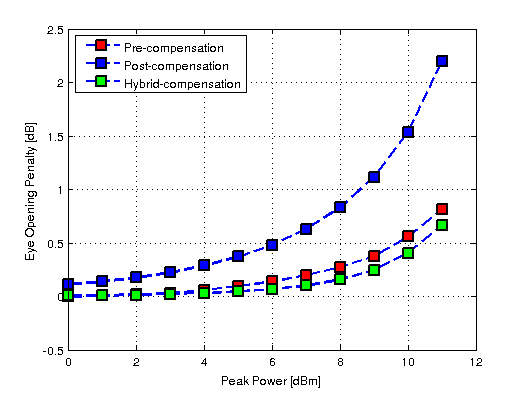
\includegraphics[width=12cm]{es5_1.png}\\
  \caption{Eye opening penalty vs peak power (without noise).}
  \label{es5_1}
\end{figure}

The hybrid-compensation scheme is the one with the lowest penalty, while the post-compensation scheme is the one with the highest penalty.


\section*{Exercise 6}
We repeat the same test in Exercise 5 but considering a noisy amplifier. In Figure \ref{es5_2} is shown the relative graph.

\begin{figure}[!ht]
  \centering
  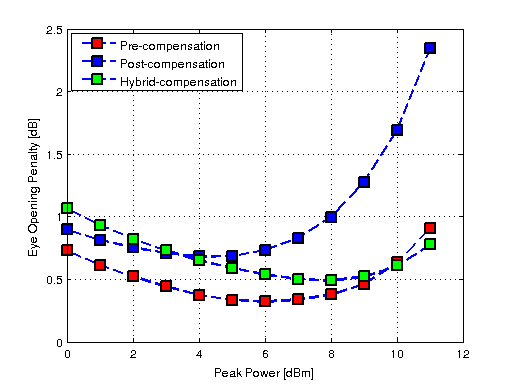
\includegraphics[width=12cm]{es5_2.png}\\
  \caption{Eye opening penalty vs peak power (with noise).}
  \label{es5_2}
\end{figure}

The penalty values are higher at the starting point respect to the previous case. They decrease until a certain power value and then they increase again.

\end{document}


\section*{Question 4}
When the power is low the eye penalty is low as well, so the performances are limited by dispersion.
When the power is high the eye penalty is high too and the performances are limited by self-phase modulation.


\section*{Question 5}
The three schemes show different performance in case of high powers because a high power causes the self-phase modulation effect. This effect
produces a chirp that generates new frequency components that propagate along the fiber and broaden the pulse spectrum.
The dispersion causes these components to propagate with different frequencies, and so, as the dispersion is different for the tree schemes, also the
penalty effect varies.
